
\section{High Availability}
\label{sec:availability}

Given the presence of network partitions and latency, systems
designers have a choice: pay the cost of possible unavailability and
potentially expensive network round-trips or seek alternative
algorithms that avoid them. Before we address the \textit{cost} of
avoiding unavailability and latency, we first need a way to classify
whether an algorithm actually incurs these penalties.

Highly available algorithms ensure ``always on'' operation and promise
a guaranteed response. If users of a highly available system contact a
(set of) replicas, then they will be \textit{available}, or able to
execute operations without having to block when replicas cannot
communicate. A useful corollary to providing high availability is
that, in the absence of failures, the system can provide a response
without having to contact other replicas and incur high
latency~\cite{abadi-pacelc}. In this section, we develop a model and
taxonomy for high availability in its various forms. This is
challenging for several reasons, including handling fault-tolerance
and, in a transactional context, handling aborts.

\subsection{Replica Availability}

Traditionally, a system provides high availability if every user that
can contact a server eventually receives a response from that server,
even in the presence of arbitrary, indefinite network partitions
between servers~\cite{gilbert-cap}. This is a useful definition: if we
can contact at least one server, then we can receive a
response. However, there are several other cases we should consider.

First, a client may wish to ensure that the effects of its operations
will persist in the face of server failure. If a client wants to
tolerate one server fault, then it should ensure that its operations
reach at least two replicas before it considers the operation
completed. According to our above definition, this $1$-fault tolerance
is not highly available; in fact, according to the above definition,
high availability is at odds with fault-tolerance! Instead, we propose
\textit{$K$-availability}: if a client can contact at least $K$
servers, then it eventually receives a response from all of
them. $1$-fault tolerance requires $2$-availability, while the
traditional ``high availability'' is equivalent to
$1$-availability. $2$-availability will require more messaging and
possibly, depending on server layout, higher latency and more
unsuccessful operations in the presence of network and server
failures.

Second, clients may wish to ensure available operation in the presence
of a minority of servers failing. This requirement is relatively
common in standard consensus algorithms like two-phase commit and
Paxos and is, by traditional standards, hardly ``highly available.''
However, it is worth acknowledging that, in an $N$ server cluster,
this \textit{majority availability} (a special case of
$K$-availability with $K=\lceil \frac{N}{2} \rceil$) provides more
frequent responses and lower latency than $N$-availability. A key
differentiation between generic $K$-availability and majority
availability is that $K$ availability is independent of the number of
servers under consideration. Fault-tolerance effectively has
``constant'' scaling cost, whereas majority availability based
algorithms are not as fortunate.

Third, clients may wish to contact the same server (or set of servers)
across subsequent operations. As we will discuss in
Section~\ref{sec:hat}, clients can ensure continuity between
operations (e.g., reading their prior updates to a data item) by
maintaining affinity or ``stickiness'' with a server or set of
servers~\cite{vogels-defs}. Ultimately, maintaining availability
during stickiness requires fate-sharing between the client and its set
of servers: if the servers a client continues to contact fail, or,
equivalently, if the client is partitioned from its designated
servers, then it may not be able to achieve its desired semantic
guarantees. We say that a system provides \textit{sticky availability}
for a user if a client's subsequent operations are executed against
the same server and, whenever the client can contact the server, it
eventually receives a response. As above, it may be useful for a
client to achieve stickiness \textit{and} fault tolerance, so we can
generalize sticky availability to \textit{$K$-sticky availability},
which provides sticky availability with $K$ distinct servers. In
certain cases, a client may wish to become $1$-sticky available by
acting as a server itself; for example, in a data store, a client
might cache its reads and writes. However, a single client cannot
achieve $K$-sticky availability with $K>1$ on its own. ``Sticking''
all clients to a designated set of servers (i.e., $K$-master
availability) is a special case of sticky availability and is less
available.

\begin{figure}
\centering
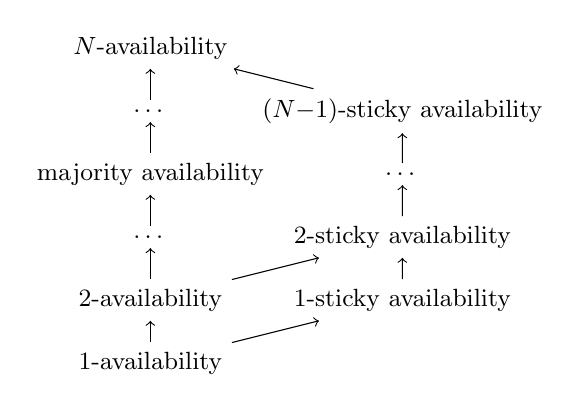
\begin{tikzpicture}[scale=0.8]
  \tikzstyle{every node}=[font=\small]
 \node[draw=none,fill=none] (1) at (0,0) {$1$-availability}; 
 \node[draw=none,fill=none] (2) at (0,1) {$2$-availability}; 
 \node[draw=none,fill=none] (m-1) at (0, 2) {\ldots}; 
 \node[draw=none,fill=none] (m) at (0, 3) {majority availability}; 
 \node[draw=none,fill=none] (m+1) at (0, 4) {\ldots}; 
 \node[draw=none,fill=none] (n) at (0, 5) {$N$-availability}; 
 \node[draw=none,fill=none] (1s) at (4, 1) {$1$-sticky availability};
 \node[draw=none,fill=none] (2s) at (4, 2) {$2$-sticky availability};
 \node[draw=none,fill=none] (n2s) at (4, 3) {\ldots};
 \node[draw=none,fill=none] (n1s) at (4, 4) {$(N$$-$$1)$-sticky availability};

 \draw [->] (1) -- (2);
 \draw [->] (2) -- (m-1);
 \draw [->] (m-1) -- (m);
 \draw [->] (m) -- (m+1);
 \draw [->] (m+1) -- (n);
 \draw [->] (1) -- (1s);
 \draw [->] (1s) -- (2s);
 \draw [->] (2) -- (2s);
 \draw [->] (2s) -- (n2s);
 \draw [->] (n2s) -- (n1s);
 \draw [->] (n1s) -- (n);


\end{tikzpicture}
\label{fig:availability-order}
\caption{Hierarchy of replica availability levels for $N>3$ servers.}
\end{figure}

We show a hierarchy of replica availabilty levels in
Figure~\ref{fig:availability-order}. $K$-availability is ``more
available'' than $K$-sticky available, but, in general, $K$-sticky
availability is incomparable with $(K+1)$-sticky
availability. However, $N$-sticky availability is effectively the same
as $N$-availability--if operations must be performed on all replicas,
then subsequent requests will trivially access the same set of
replicas.

There are three further aspects of replica availability that deserve
mention. First, availability may be decomposed into operation-specific
levels. For instance, many quorum-based replication systems allow for
tuning based on workload and desired performance; a read-one,
write-all (ROWA) quorum-replicated data store would experience
$N$-availability for writes but $1$-availability for reads. Second, we
have assumed that server membership in the system is static. In
practice, servers may join and leave a deployment over time. Aside
from setting $N=\infty$, systems may wish to reevaluate their
algorithm choice, particularly for $N$ and majority available
algorithms. Third, in many deployments, such as a data store, a given
set of operations may be logically restricted to a subset of the
servers in the cluster. In a partitioned database, the only servers
who perform read and write operations are typically those that are
designed as replicas for a given item. Accordingly, $N$ is determined
by the replication factor of the data store (e.g., three to five) as
opposed to the number of servers comprising the data store (e.g., tens
to thousands). In this paper, we do not focus on further
taxonomization of replica availability (e.g., within versus across
datacenters) but believe there is worthwhile future work in doing so.

\subsection{Transactional Availability}

Thus far, we have focused on single-operation availability. This is
standard in distributed systems literature (e.g., atomic, regular, and
safe register models all concern single objects), yet the database
literature largely focuses on transactions: groups of multiple
operations over multiple objects. Replica availability alone is
insufficient to describe availability guarantees for
transactions. Additionally, given the choice of \textit{commit} and
\textit{abort} responses---which signal transaction success or failure
to a client---we must be careful in defining availability.

First, if a client wishes to execute a transaction that performs
operations on $D$ distinct data items that are spread across servers,
then it must be able to contact servers for those data items. This is
different from, say, $1$-replica availability or $D$-replica
availability; instead, the client requires a degree of replica
availability for \textit{each} respective data item. This this
\textit{transactional requirement for replica availability} may result
in lower availability than a non-transactional requirement (e.g.,
requesting from two servers instead of one for a two-item transaction)
but not necessarily (e.g., both items in a two-item transaction are
located on the same server).

Second, given the possiblity of aborts, we need to ensure useful
forward progress. A system can trivially guarantee clients a response
by always aborting their
transactions~\cite{transaction-liveness}. However, this is an
unsatisfactory system because nothing good (transaction commit) ever
happens; instead, we require a \textit{liveness} property. We cannot
guarantee that every transaction will commit---transactions may choose
to abort themselves---but we need to make sure that the system will
not indefinitely abort transactions on its own volition. We call a
transaction abort due to a transaction's own choosing (e.g., as part
of the transaction itself or due to a would-be integrity constraint
violation) an \textit{internal abort} and an abort due to system
implementation an \textit{external abort}.

We say that a system provides \textit{transactional availability} if,
given replica availability for every data item in a transaction, the
transaction eventually commits or internally aborts. For example,
system will violate transactional $2$-availability if client that can
contact two servers for each of four data items in its transaction
cannot eventually commit in the absence of internal aborts.

\subsection{Discussion}

In order to provide a framework in which to evaluate partition and
latency sensitivity, we have introduced a taxonomy of replica and
transactional availability requirements. The many variants of this
taxonomy are interesting on their own, but, given our goal, two models
stand out as particularly useful.

$1$-availability is the standard model for ``high availability'' in a
distributed environment. Any system purporting to be ``highly
available'' today is---if it is
honest---$1$-available. $1$-availability is particularly useful as it
means that \textit{any} server (or, in the case of a database system,
replica) can handle a request. This is particularly strong:
availability is guaranteed unless a client is partitioned from
\textit{all} servers and, aside from latency associated with
contacting the server to begin with, requests can complete effectively
locally. This mitigates many of the costs of the distributed
model---albeit at the expense of semantic guarantees
(Section~\ref{sec:hats}). $1$-sticky availability is also fairly
common and is often cited as a technique for cheaply providing several
useful guarantees, like the aforementioned ``read your writes''
guarantees.

In this work, we will focus on developing the theory of $1$-available
and $1$-sticky available systems. While it is possible to provide low
latency in addition to higher $K$-availability and $K$-sticky
availabililty (e.g., for fault tolerance via increased server count
within a given datacenter), we reserve this exploration for future work.

